
%*******************************************
% Author:      se7enlcd                    *
% E-mail:      2353442022@qq.com           *
% Date:        2023-06-02                  *
% Description:                             *
%*******************************************


\documentclass[a4paper, 10pt]{report}
\usepackage[hyperref=true, backend=bibtex, sorting=none, backref=true]{biblatex} %style=authoryear-icomp
\usepackage[dvipsnames, svgnames, x11names]{xcolor}
\usepackage[a4paper, left=1.5cm, right=1cm, top=1.5cm, bottom=1.5cm]{geometry}
\usepackage{tocloft} % 目录设置宏包
\usepackage{enumerate}
\usepackage{fontspec, xunicode-addon} % 显示中文、韩文(CJK)字符
\usepackage[utf8]{inputenc}
\usepackage{kotex} % korea font space
\usepackage{multicol}
\usepackage{verse} % 诗歌
\usepackage[fleqn]{amsmath}
\usepackage{etoolbox}
\usepackage{amsfonts}
\usepackage{amssymb}
\usepackage{pifont} % \ding{51}
\usepackage[runin]{abstract}
\usepackage{lipsum} % 插入例子
\usepackage{xifthen}
\usepackage{tcolorbox}
\usepackage{enumitem}
\usepackage{tasks}
\usepackage{graphicx}
\usepackage{tabularray}
\usepackage[slantfont, boldfont]{xeCJK}
\usepackage{titling}
\usepackage[explicit]{titlesec}
\usepackage{metalogo}
\usepackage{chngcntr}
\usepackage{fontawesome5}
\usepackage{IEEEtrantools}
\usepackage{newclude}
\usepackage{minted} % sudo pip install pygments % --shell-escape
\usepackage[titletoc]{appendix} % 附录
\usepackage{todonotes} % 批注将来需要做的事项
\usepackage[noautomatic]{imakeidx} % 关键字索引 导言区\index{}
\usepackage[totoc, hangindent=2em, subindent=0.8em, initsep=12pt, font=small, unbalanced=true]{idxlayout}
\usepackage{pst-plot}
\usepackage[customcolors, shade]{hf-tikz}
\usetikzlibrary{tikzmark}
\usepackage{tkz-euclide}
\usepackage{codebox}
\usepackage{fancyhdr} % 设置页眉、页脚
\usepackage{lastpage} % 显示总页数
\usepackage{afterpage}
\usepackage{hyperref} % 此宏包必须最后导入才能跳转到引用位置

\usemintedstyle{xcode}

% --------------------------------------------------------
% -------------- input sources file begin ----------------
% --------------------------------------------------------
% Chinese
\setmainfont{Times New Roman}
\defaultCJKfontfeatures{Scale=0.9}
\setCJKmainfont[ItalicFont={KaiTi}, BoldFont={Microsoft YaHei}]{KaiTi} %衬线字体 缺省中文字体为宋体
\setCJKsansfont{Microsoft YaHei} %serif是有衬线字体sans serif无衬线字体。
\setCJKmonofont{FangSong} %中文等宽字体

% Korea
% \setCJKfamilyfont{korm}{Gowun Batang}
\setCJKfamilyfont{korm}{NanumMyeongjo}
\newcommand\krt{\CJKfamily{korm}\CJKspace\footnotesize} % footnotesize small normalsize
\newcommand\kr{\CJKfamily{korm}\CJKspace\normalsize} % footnotesize small normalsize

%  NOTE:  XeLaTeX 下需要把全体带圈数字都设置成 Default 类
\xeCJKDeclareCharClass{Default}{"24EA, "2460->"2473, "3251->"32BF}
\newfontfamily\EnclosedNumbers{Source Han Serif CN} % NOTE: adobe
\AtBeginUTFCommand[\textcircled]{\begingroup\EnclosedNumbers}
\AtEndUTFCommand[\textcircled]{\endgroup}

%--------------------添加本地系统内的中文字体---------------------
\setCJKfamilyfont{song}{SimSun}           % 宋体
\newcommand{\song}{\CJKfamily{song}}      % 宋体
\setCJKfamilyfont{kaiti}{KaiTi}           % 楷体
\newcommand{\kaiti}{\CJKfamily{kaiti}}    % 楷体
\setCJKfamilyfont{fsong}{FangSong}        % 仿宋
\newcommand{\fsong}{\CJKfamily{fsong}}    % 仿宋
\setCJKfamilyfont{hei}{SimHei}            % 黑体
\newcommand{\hei}{\CJKfamily{hei}}        % 黑体
\setCJKfamilyfont{yh}{Microsoft YaHei}    % 微软雅黑
\newcommand{\yh}{\CJKfamily{yh}}          % 微软雅黑

%------------------------------设置字体大小------------------------
\newcommand{\chuhao}{\fontsize{42pt}{\baselineskip}\selectfont}     %初号
\newcommand{\xiaochuhao}{\fontsize{36pt}{\baselineskip}\selectfont} %小初号
\newcommand{\yihao}{\fontsize{28pt}{\baselineskip}\selectfont}      %一号
\newcommand{\erhao}{\fontsize{21pt}{\baselineskip}\selectfont}      %二号
\newcommand{\xiaoerhao}{\fontsize{18pt}{\baselineskip}\selectfont}  %小二号
\newcommand{\sanhao}{\fontsize{15.75pt}{\baselineskip}\selectfont}  %三号
\newcommand{\sihao}{\fontsize{14pt}{\baselineskip}\selectfont}      %四号
\newcommand{\xiaosihao}{\fontsize{12pt}{\baselineskip}\selectfont}  %小四号
\newcommand{\wuhao}{\fontsize{10.5pt}{\baselineskip}\selectfont}    %五号
\newcommand{\xiaowuhao}{\fontsize{9pt}{\baselineskip}\selectfont}   %小五号
\newcommand{\liuhao}{\fontsize{7.875pt}{\baselineskip}\selectfont}  %六号
\newcommand{\qihao}{\fontsize{5.25pt}{\baselineskip}\selectfont}    %七号

%------------------------------标题名称中文化---------------------
\renewcommand\abstractname{\kaiti 摘\ 要}
\renewcommand\abstracttextfont{\kaiti}
\setlength\absleftindent{0pt}
\setlength\absrightindent{0pt}
\setlength{\abstitleskip}{-1.5em} % 调整摘要与正文之间的距离,默认为上下加runin参数后变为左右距离
\abslabeldelim{:}

\renewcommand\figurename{\hei 图}

% 章节标题格式设置
\titleformat
{\chapter}                  % 章节命令
% [display]                 % shape
{\kaiti\LARGE\centering\color{black}}  % 章节字体格式
{第 \thechapter 章}                          % 章节数字前缀
{0.5ex}                       % 前缀与题目之间的间距
{#1}                          % 设置题目本身格式
[]         % 章节后缀(后最内容会出现在章节的下方)

\titleformat
{\section}                  % 章节命令
{\kaiti\Large\raggedright\color{BrickRed}}  % 章节字体格式
{\faIcon{toggle-on}}                          % 章节数字前缀
{5pt}                       % 前缀与题目之间的间距
{#1  \textcolor{black}{\faIcon{github}} \textcolor{blue}{\faIcon{code}} \textcolor{black}{\faIcon{pen-nib}} \textcolor{red}{\faIcon{terminal}}}                          % 设置题目本身格式
[{\titlerule[2pt]}]         % 章节后缀(后最内容会出现在章节的下方)


\titleformat
{\subsection}                  % 章节命令
{\kaiti\large\raggedright\color{RoyalBlue}}  % 章节字体格式
{\faIcon{tag}}                          % 章节数字前缀
{5pt}                       % 前缀与题目之间的间距
{#1}                          % 设置题目本身格式
%[{\titlerule[2pt]}]         % 章节后缀(后最内容会出现在章节的下方)


% ------------ 目录格式设置 -------------
% \usepackage{tocloft}
% TOC title name chage
\renewcommand{\cftbeforetoctitleskip}{0pt}
\renewcommand{\cftaftertoctitleskip}{1.8cm}
\renewcommand{\contentsname}{目录}
\renewcommand{\cfttoctitlefont}{\kaiti \huge \bfseries \hfill} % content 居中对齐
\renewcommand{\cftaftertoctitle}{\hfill \kaiti} % content 居中对齐

% contents table name chage
\renewcommand{\cftbeforelottitleskip}{0pt}
\renewcommand{\cftafterlottitleskip}{1.8cm}
\renewcommand{\listtablename}{表格目录}
\renewcommand{\cftlottitlefont}{\kaiti \huge \hfill \bfseries} % content 居中对齐
\renewcommand{\cftafterlottitle}{\hfill \kaiti} % content 居中对齐
\renewcommand{\cfttabindent}{0pt} % table 缩进

% contents figure name chage
\renewcommand{\cftbeforeloftitleskip}{0pt}
\renewcommand{\cftafterloftitleskip}{1.8cm}
\renewcommand{\listfigurename}{图片目录}
\renewcommand{\cftloftitlefont}{\kaiti \huge \hfill \bfseries} % content 居中对齐
\renewcommand{\cftafterloftitle}{\hfill \kaiti} % content 居中对齐
\renewcommand{\cftfigindent}{0pt} % figure 缩进

%------------- chapter 格式设置 ----------
\renewcommand{\cftbeforechapskip}{10pt}
\renewcommand{\cftchapfont}{\large \kaiti\bfseries}     % chapter 格式设置
\renewcommand{\cftchappresnum}{第}     % chapter 格式设置
\renewcommand{\cftchapaftersnum}{章}     % chapter 格式设置
% \renewcommand{\cftchapaftersnumb}{\newline}     % chapter 格式设置
\renewcommand{\cftchapnumwidth}{1.8cm}     % chapter 格式设置


%------------- section 格式设置 ----------
\renewcommand{\cftsecfont}{\normalsize}     % section 格式设置
\renewcommand{\cftsecindent}{0.74cm}
\renewcommand{\cftsecnumwidth}{1.05cm}     % section 格式设置

%------------- subsection 格式设置 ----------
\renewcommand{\cftsubsecindent}{1.65cm}
\renewcommand{\cftsubsecnumwidth}{1cm}     % section 格式设置
\renewcommand{\cftsubsecfont}{\normalsize}     % subsection 格式设置


% 目录深度4, 从0开始
\setcounter{tocdepth}{3}

\renewcommand{\cftchapdotsep}{\cftdotsep}
\renewcommand{\cftchapleader}{
	% \renewcommand{\cftdot}{-}
	\cftdotfill{\cftchapdotsep}
}

\renewcommand{\cftfigindent}{0pt}
\renewcommand{\cftpnumalign}{c}

%*******************************************
% Author:      lcdse7en                    *
% E-mail:      2353442022@qq.com           *
% Date:        2023-05-04                  *
% Description:                             *
%*******************************************

% latex内置了四种页眉、页脚的样式:empty(没有页眉和页脚)、plain(没有页眉,页脚中部放置页码)、headings(没有页脚,页眉包含章节的标题和页码)
% \usepackage{fancyhdr} 自定义页眉和页脚
\fancypagestyle{mypagestyle}{        % RO: 右边奇数页 ;LE:左边偶数页
	\fancyhead{}
	\fancyfoot{}
	% renewcommand{\thepage}{\arabic{page}} % part chapter section equation page figure table
	% setcount{page}{1}
	\fancyhead[LE,RO]{\thepage}
	\fancyhead[RE]{\leftmark}          % 获取当前页所在章的标题
	\fancyhead[LO]{\rightmark}         % 获取当前页所在节的标题
	\fancyfoot[CO,CE]{\thepage / \pageref{LastPage}} % 获取最后一页的页码(需要\usepackage{lastpage}宏包)
	\renewcommand{\headrulewidth}{0.8pt}
	\renewcommand{\footrulewidth}{0pt}
}
\fancypagestyle{plain}{        % RO: 右边奇数页 ;LE:左边偶数页
	\fancyhead{}
	\fancyfoot[CO, CE]{\thepage}
	% renewcommand{\thepage}{\arabic{page}} % part chapter section equation page figure table
	% setcount{page}{1}
	\renewcommand{\headrulewidth}{0pt}
	\renewcommand{\footrulewidth}{0pt}
}


\setlength\headwidth{\textwidth}

% ----------- enumerate setting -------------
\setlist[enumerate, 1]{
	label = {\arabic*.},
	labelindent=\parindent,
	leftmargin=*,
}
\setlist[enumerate, 2]{
	% label = \emph{(\arabic*).},
	label = {(\arabic*)},
	topsep = 0pt,
	labelindent=2pt,
	leftmargin=*,
}
\setlist[enumerate, 3]{
	label = \emph{\arabic*).},
	topsep = 0pt,
	labelindent=2pt,
	leftmargin=*,
}

%*******************************************
% Author:      lcdse7en                    *
% E-mail:      2353442022@qq.com           *
% Date:        2023-05-04                  *
% Description:                             *
%*******************************************

\newcommand{\imp}[1]{\underline{\textit{#1}}}  % 下划线强调


\newlist{todolist}{itemize}{2}
\setlist[todolist]{label=$\square$}
% for check symbol
% \usepackage{pifont}
\newcommand{\cmark}{\ding{51}}%
\newcommand{\xmark}{\ding{55}}%
\newcommand{\done}{\rlap{$\square$}{\raisebox{2pt}{\large\hspace{1pt}\cmark}}\hspace{-2.5pt}}
\newcommand{\wontfix}{\rlap{$\square$}{\large\hspace{1pt}\xmark}}

% Bibnatg Commands
\newcommand{\hlmath}[2]{\colorbox{#1!17}{$\displaystyle #2$}}
\newcommand{\hltext}[2]{\colorbox{#1!17}{#2}}





% \begin{itemize}
% 	\item 2019年9月30日计划
% 	\begin{todolist}
% 		\item [\wontfix] 休息休息
% 		\item [\done] 吃饭
% 		\item [\done] 学习
% 		\item 8点开始学习。
% 		\item 待完成。。。
% 	\end{todolist}
% \end{itemize}

\newcommand*{\circled}[1]{\lower.7ex\hbox{\tikz\draw (0pt, 0pt)
		circle (.5em) node {\makebox[1em][c]{\small #1}};
	}}
\robustify{\circled}
\NewTasksEnvironment[style=enumerate,
	label=$\Alph*$.,
	label-width=13pt,
	after-item-skip=0ex
]{choice}[\item]
\NewTasksEnvironment[style=enumerate,
	% label=\large\protect\textcircled{\arabic*},
	label=\circled{\arabic*},
	label-width=12pt,
	after-item-skip=0ex
]{stage}[\item]

% --------------------------------------------------------
% ------------------ basec-info image -------------------
% --------------------------------------------------------
\newcommand{\pdf}{
\includegraphics[height=.85em]{png/pdf.png}}
\newcommand{\gh}{
\includegraphics[height=.85em]{png/gh.png}}
\newcommand{\www}{
\includegraphics[height=.85em]{png/www.png}}
\newcommand{\email}{
\includegraphics[height=.85em]{png/email.png}}
\newcommand{\gitee}{
\includegraphics[height=.85em]{png/gitee.png}}
\newcommand{\rufus}{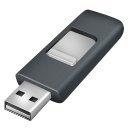
\includegraphics[height=.85em]{png/rufus.png}}
\newcommand{\wechat}{
\includegraphics[height=.85em]{png/wechat.png}}
\newcommand{\phone}{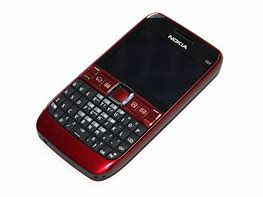
\includegraphics[height=.85em]{png/phone.png}}


%*******************************************
% Author:      lcdse7en                    *
% E-mail:      2353442022@qq.com           *
% Date:        2023-05-03                  *
% Description:                             *
%*******************************************

\graphicspath{ {./images/} }

% --------------------------------------------------------
% -------------------- 自定义颜色 ------------------------
% --------------------------------------------------------
% https://coolors.co/

\definecolor{mygrey}{RGB}{128,128,128}
\definecolor{myteal}{RGB}{0,128,128}
\definecolor{mypink}{RGB}{250,218,221}
\definecolor{mygray}{gray}{0.9}
\definecolor{mypage}{HTML}{048fdf}
\definecolor{mychinarose}{HTML}{b56576}

% --------------------------------------------------------
% ----------- setting Table environment start --------------
% --------------------------------------------------------
\NewTblrEnviron{mytblr}
\SetTblrOuter[mytblr]{long}
\SetTblrInner[mytblr]{
	width = 0.99\linewidth,
	rowhead = 1,
	verb,
	row{odd} = {bg=mypink},
	row{1} = {bg=myteal, fg=white},
}


\SetTblrInner[longtblr]{
	cells = {font=\small},
	rowhead = 1,
	cell{1}{-} = {fg=white, bg=gray, font=\bfseries\kaiti\small}
}

\SetTblrStyle{caption, note, remark}{font=\small}
\SetTblrStyle{caption-tag}{red2}
\SetTblrStyle{firstfoot, middlefoot, lastfoot}{fg=blue2, font=\kaiti\small}
\SetTblrStyle{firsthead, middlehead, lasthead}{font=\bfseries\kaiti\small}

\UseTblrLibrary{counter}
\newcounter{mycnta}
\newcommand{\mycnta}{\stepcounter{mycnta}\arabic{mycnta}}
\counterwithin{mycnta}{table} % page\ table
\renewcommand\themycnta{\arabic{mycnta}}

\NewTableCommand\myhline{\hline[0.2em,black]}

\DeclareTblrTemplate{caption-sep}{default}{\enskip}
\DeclareTblrTemplate{contfoot-text}{default}{(接下页)}
\DeclareTblrTemplate{conthead-text}{default}{(续前表)}


\UseTblrLibrary{booktabs} % 三线表库 \toprule \midrule \bottomrule \cmidrule
\UseTblrLibrary{amsmath}
\UseTblrLibrary{diagbox} % 斜线标头库 \diagbox{}{} \diagboxthree{}{}{}
\UseTblrLibrary{siunitx}
% --------------------------------------------------------
% ----------- setting Table environment end --------------
% --------------------------------------------------------

%*******************************************
% Author:      lcdse7en                    *
% E-mail:      2353442022@qq.com           *
% Date:        2023-05-04                  *
% Description:                             *
%*******************************************

\hypersetup{
    colorlinks=true,
    linkcolor = black, % 目录颜色
    urlcolor=Blue,
    citecolor=Cyan,
    filecolor=Green,
    pdfview=XYZ,
}

\let\oldhref\href
\renewcommand{\href}[3][blue]{\oldhref{#2}{\color{#1}{#3}}}

\newtcbox{\xmybox}[1][red]{
	on line,
	arc=6pt,
	colback=#1!10!white,
	colframe=#1!50!black,
	before upper={\rule[-1.5pt]{0pt}{10pt}},
	boxrule=1pt,
	boxsep=0pt,
	left=8pt,
	right=8pt,
	top=1pt,
	bottom=1pt
}

% 两列以及同高度的tcolorbox
\newtcolorbox{mybox2}[2]{
	width=(\linewidth-2mm)/2,
	nobeforeafter,
	arc=1mm,
	coltitle=black,            % title字体颜色
	colbacktitle=red!50!white, % title背景颜色
	colback=yellow!50!red!25!white, % 内容背景颜色
	colframe=blue!75!black,    % 边框颜色
	fonttitle=\bfseries,
	fonttitle=\kaiti,
	fontupper=\kaiti,
	left=2mm, % 内容与左边边框的间距
	right=2mm,
	top=1mm,
	bottom=1mm,
	title= #1,
	equal height group=#2,    % parbox
}


\newtcblisting[auto counter]{mypython}[1]{
	minted style=xcode,
	minted language=python,
	listing engine=minted,
	minted options={
			linenos,
			autogobble,
			% gobble=2,
			mathescape,
			fontsize=\small,   % large, normalsize, small, footnotesize
			breaklines,
			highlightcolor=yellow!50,
			% #2,  % highlightlines={1,4},
			bgcolor=mygray,
			numbersep=3mm
		},
	colback=yellow!5,
	colframe=yellow!50!black,
	% fonttitle=\bfseries,
	listing only,
	left=5mm,
	enhanced,
	overlay={\begin{tcbclipinterior}\fill[red!10!blue!13!white] (frame.south west)
				rectangle ([xshift=5mm]frame.north west);\end{tcbclipinterior}},
	title={\textcolor{yellow}{\bfseries Code \thetcbcounter:} #1},
	top=0mm,
	bottom=0mm,
	after title=\hfill\textcolor{red}{\faIcon{python}PYTHON}
}


\newtcblisting[auto counter]{mytex}[1]{
	listing engine=minted,
	minted style=xcode,
	minted language=latex,
	minted options={
			linenos,
			autogobble,
			% gobble=2,
			mathescape,
			fontsize=\small,   % large, normalsize, small, footnotesize
			breaklines,
			highlightcolor=yellow!50,
			% #2,  % highlightlines={1,4},
			bgcolor=mygray,
			numbersep=3mm
		},
	colback=yellow!5,
	colframe=yellow!50!black,
	% fonttitle=\bfseries,
	listing only,
	left=5mm,
	enhanced,
	overlay={\begin{tcbclipinterior}\fill[red!10!blue!13!white] (frame.south west)
				rectangle ([xshift=5mm]frame.north west);\end{tcbclipinterior}},
	title={\textcolor{yellow}{\bfseries Code \thetcbcounter:} #1},
	top=0mm,
	bottom=0mm,
	after title=\hfill \textcolor{black}{\faIcon{pen-nib} LaTex}
}



\newtcblisting[auto counter]{mysh}[1]{
	listing engine=minted,
	minted style=xcode,
	minted language=shell,
	minted options={
			linenos,
			autogobble,
			% gobble=2,
			mathescape,
			fontsize=\small,   % large, normalsize, small, footnotesize
			breaklines,
			highlightcolor=yellow!50,
			% #2,  % highlightlines={1,4},
			bgcolor=mygray,
			numbersep=3mm
		},
	colback=yellow!5,
	colframe=yellow!50!black,
	% fonttitle=\bfseries,
	listing only,
	left=5mm,
	enhanced,
	overlay={\begin{tcbclipinterior}\fill[red!10!blue!13!white] (frame.south west)
				rectangle ([xshift=5mm]frame.north west);\end{tcbclipinterior}},
	title={\textcolor{yellow}{\bfseries Code \thetcbcounter:} #1},
	top=0mm,
	bottom=0mm,
	after title=\hfill \textcolor{black}{\faIcon{terminal} Shell}
}


\newcounter{filePrg}
\newtcbinputlisting[use counter=filePrg, number within=chapter, list inside=mypyg]{\inputcodefile}[5]{
	listing engine=minted,
	minted style=xcode,
	minted language=#1,
	listing file={#2},
	minted options={
			linenos,
			% bgcolor=mygray,
			fontsize=\small,   % large, normalsize, small, footnotesize
			breaklines,
			autogobble,
			numbersep=3mm,
			mathescape,
		},
	breakable,
	arc=1.5mm,
	colframe=brown,
	% colback=yellow!5,
	coltitle=White,
	coltext=Black,
	listing only,
	size=title,
	% drop fuzzy shadow,
	left=5mm,
	enhanced,
	% overlay={\begin{tcbclipinterior}\fill[red!20!blue!20!white] (frame.south west)
	% 			rectangle ([xshift=5mm]frame.north west);\end{tcbclipinterior}},
	top=0mm,
	bottom=0mm,
	interior style={
			fill overzoom image=images/#5,
			fill image opacity=0.49,
		},
	% frame style image=001.jpeg,
	% watermark text app={\textit{Se7en}},
	% watermark color=Navy,
	% watermark opacity=0.10,
	title={\textcolor{yellow}{\bfseries Listing \thetcbcounter:} #3},
	list entry=Listing~\thetcbcounter : #3,
	after title=\hfill \textcolor{black}{\faIcon{pen-nib} #4},
	% label=lst:#4
}

% Making the \entry command
\newcommand{\entry}[4]{
	\ifthenelse{\isempty{#3}}
	{\slimentry{#1}{#2}}{

		\begin{minipage}[t]{.15\linewidth}
			\hfill \textsc{#1}
		\end{minipage}
		\hfill\vline\hfill
		\begin{minipage}[t]{.78\linewidth}
			% {\bf#2}\\\textit{#3} \footnotesize{#4}
			% large normalsize small footnotesize
			% DarkOliveGreen LightSlateGrey DarkCyan
			{\bf#2}\\\small\textcolor{DarkCyan}{#3} \small{#4}
		\end{minipage}\\
		\vspace{.25cm}
	}}

\newcommand{\slimentry}[2]{

	\begin{minipage}[t]{.15\linewidth}
		\hfill \textsc{#1}
	\end{minipage}
	\hfill\vline\hfill
	\begin{minipage}[t]{.78\linewidth}
		\small#2
	\end{minipage}\\
	\vspace{.25cm}
}% end \entry command definition

\newcommand{\attrib}[1]{%
  \nopagebreak{\raggedleft\footnotesize #1\par}
}

\setlength{\columnseprule}{1pt}
% \def\columnseprulecolor{\color{blue}}
\def\columnseprulecolor{\color{mypink}}


%*******************************************
% Author:      lcdse7en                    *
% E-mail:      2353442022@qq.com           *
% Date:        2023-05-03                  *
% Description:                             *
%*******************************************

\addbibresource{bibliography/ref.bib}


%*******************************************
% Author:      lcdse7en                    *
% E-mail:      2353442022@qq.com           *
% Date:        2023-05-04                  *
% Description:                             *
%*******************************************

\makeindex[
    columns=2,
    title={中文索引},
    intoc, % 将索引的标题添加到目录之中
    columnseprule=true, % 列之间添加垂直线
    columnsep=5pt,
    options = {-s zh.ist}
]

% --------------------------------------------------------
% --------------- input sources file end -----------------
% --------------------------------------------------------

% ---------------- begin document start ------------------
\begin{document}

\pagestyle{mypagestyle}


%*******************************************
% Author:      lcdse7en                    *
% E-mail:      2353442022@qq.com           *
% Date:        2023-05-04                  *
% Description:                             *
%*******************************************


\begin{titlepage}
	\thispagestyle{empty}
	\begin{tikzpicture}[remember picture, overlay]
		\draw[fill=mypage] (current page.north west) rectangle (current page.south east);

		\node[anchor=north west, xshift=-0.1cm, yshift=1cm] (bg) at (current page.north west) {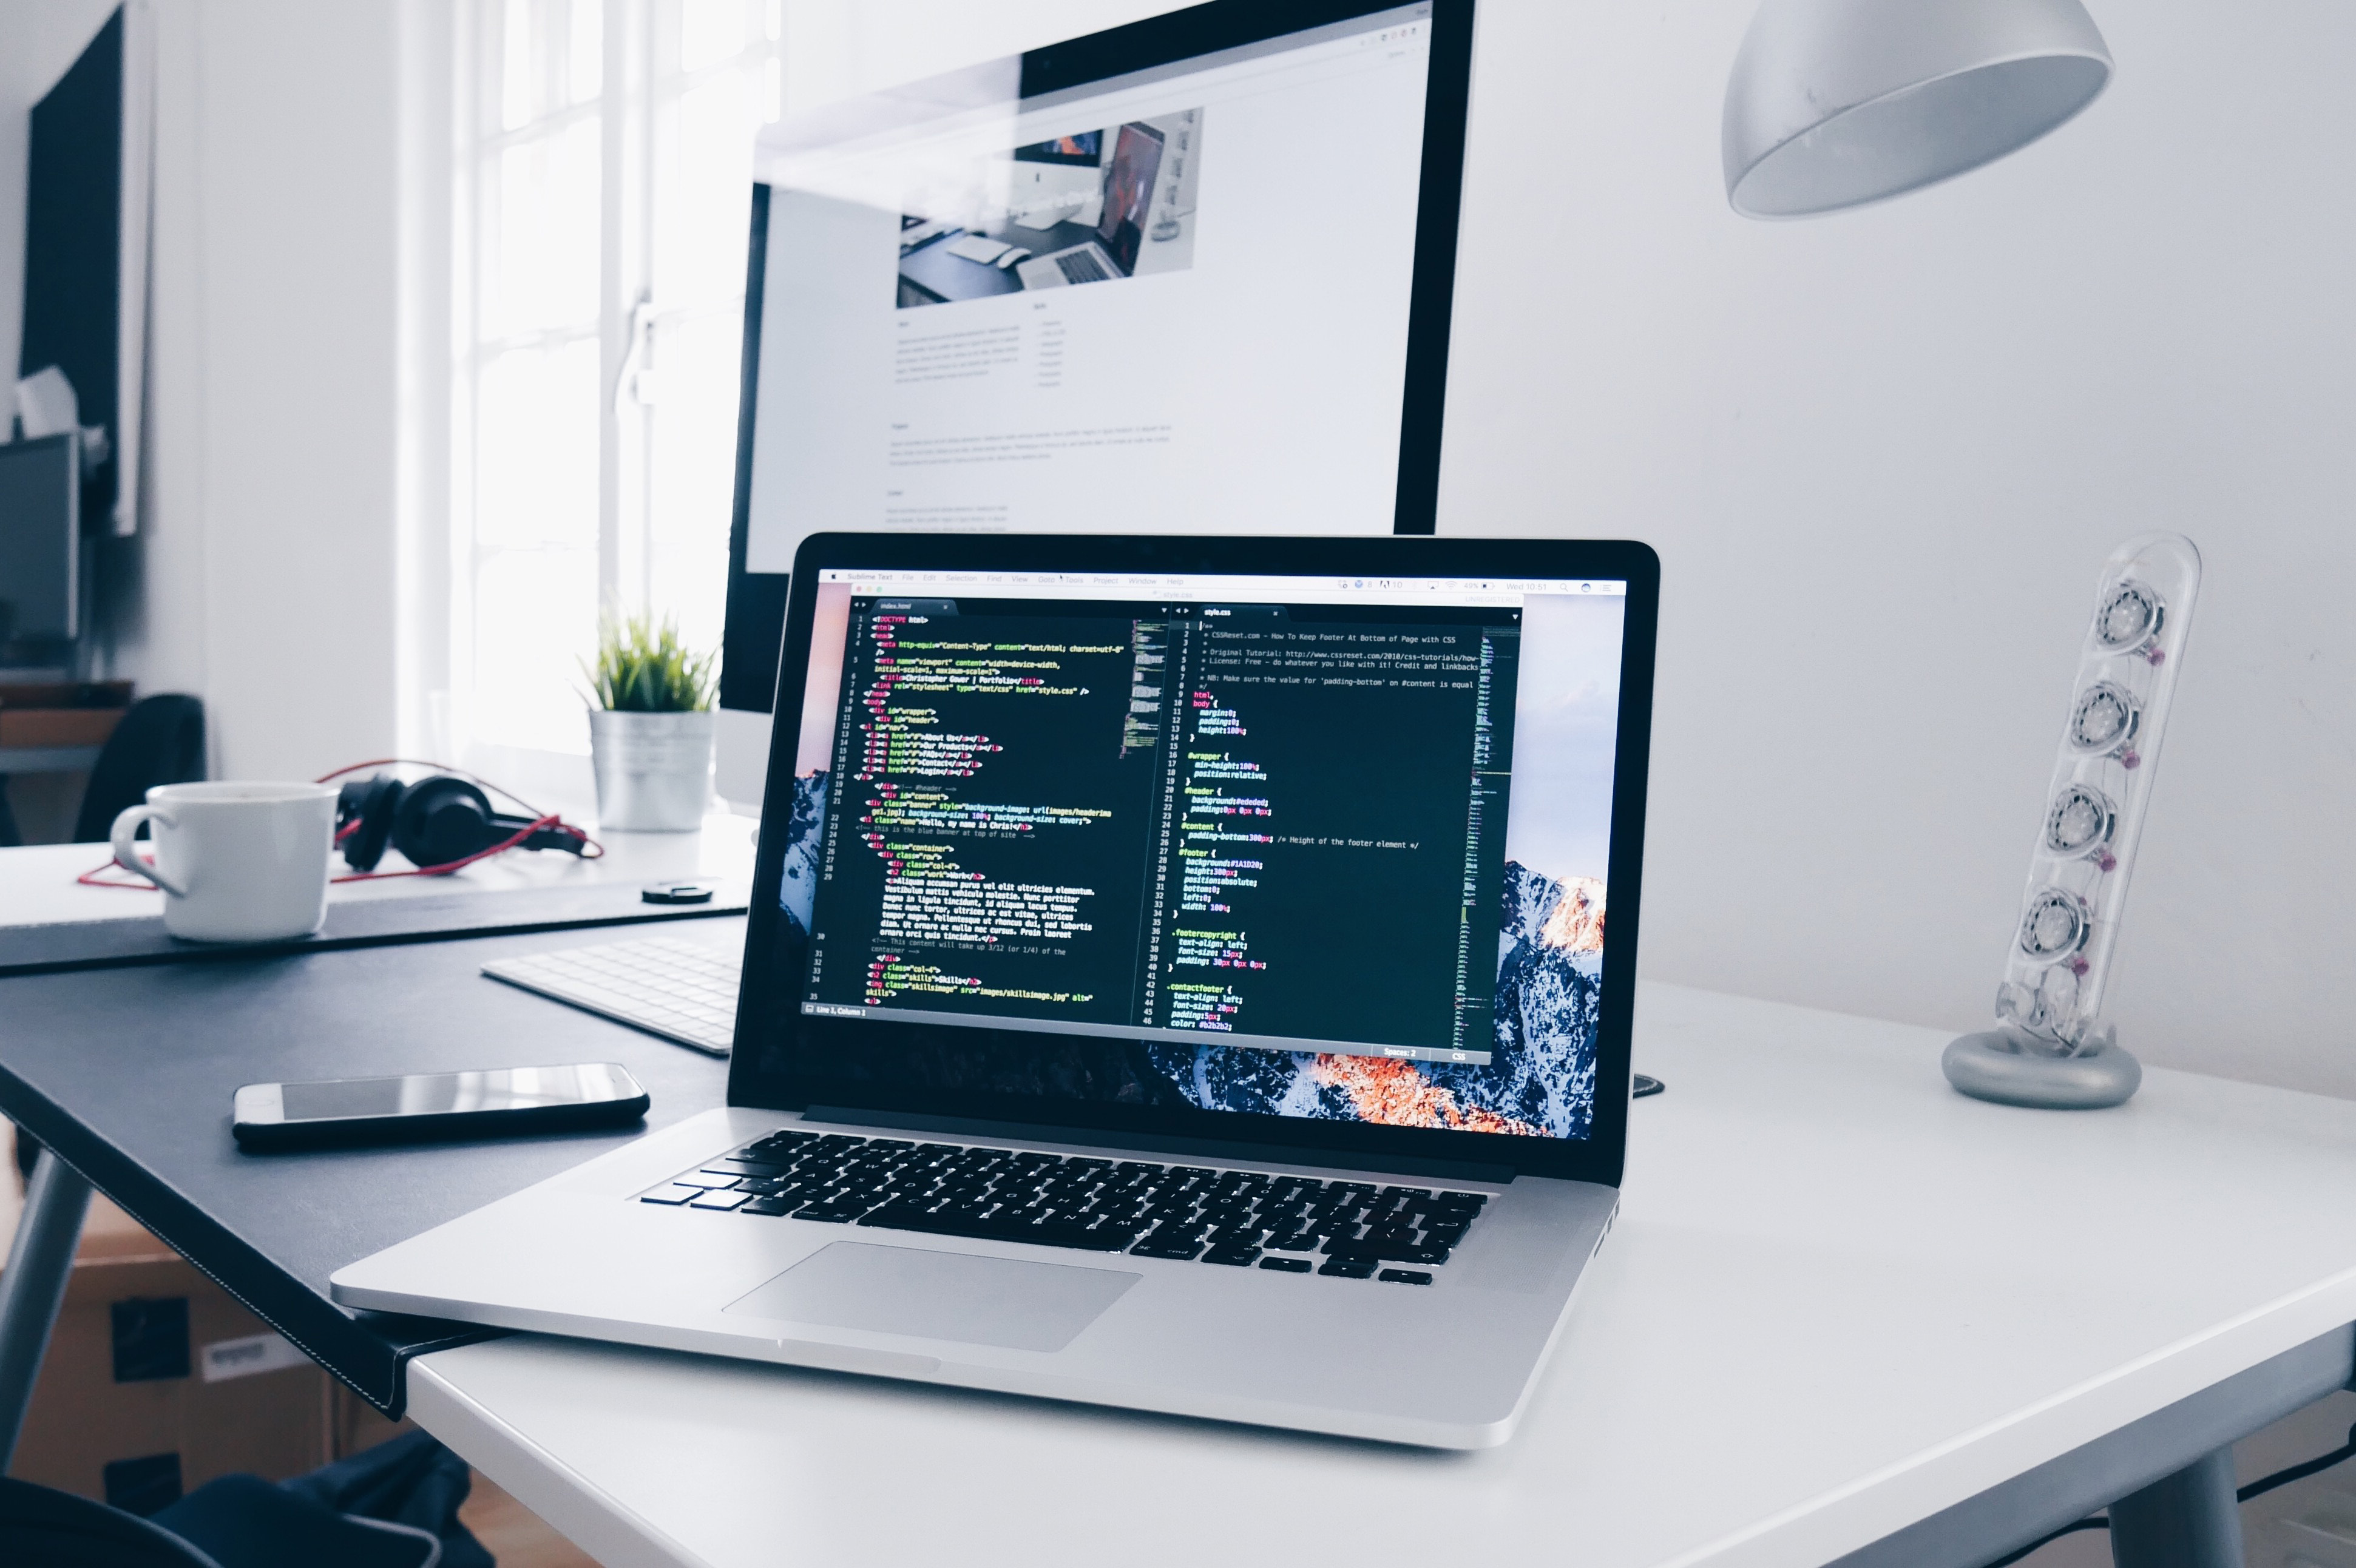
\includegraphics[width=\paperwidth, height=15cm]{title1.jpeg}};

		\node[anchor=west, text width=\textwidth, color=white, below=of bg] (title) {\LARGE\kaiti LaTex};

		\node[inner sep=0.25cm, text width=25cm, color=white, below=of title, fill=white, text=black!70, yshift=-1cm] at
		(current page.east) (subtitle) {\LARGE\kaiti\bfseries CTAN Packages};


		\node[anchor=west, text width=\textwidth, color=white, below=of title, yshift=-6cm] (date) {\LARGE\today};
		\node[anchor=west, text width=\textwidth, color=white, below=of date] (add) {\LARGE Shenzhen, China};

		\node[fill=white, draw=white, minimum width=7cm, below=of add, anchor=west] at (add.west) (line) {};

		\node[anchor=west, text width=\textwidth, color=white, below=of line, anchor=west] at (line.west) (author) {\LARGE Authored By: Se7enlcd};
	\end{tikzpicture}
\end{titlepage}
 % 封面页面

\thispagestyle{empty}
\afterpage{\thispagestyle{plain}}
\renewcommand{\thepage}{\Roman{page}}
\setcounter{page}{1}
\tableofcontents

\clearpage
\listoftables % 表格目录

\clearpage
\listoffigures % 图片目录

%\listoftodos
\newpage

%\begin{minipage}[t]{.5\linewidth}
	\begin{tabular}{rp{.75\linewidth}}
		\baselineskip=20pt
		\email{} : & \href{2353442022@qq.com}{2353442022@qq.com}                                               \\
		\www{}   : & \href{https://mirrors.tuna.tsinghua.edu.cn/archlinux/iso/latest/}{Archlinux iso Download}
	\end{tabular}
\end{minipage}
\begin{minipage}[t]{.5\linewidth}
	\begin{tabular}{rl}
		\gh{}    :    & \href{https://github.com/lcdse7en/archlinux}{https://github.com/lcdse7en/archlinux} \\
		\wechat{}   : & \href{se7enlcd}{se7enlcd}
	\end{tabular}
\end{minipage}

%% \renewcommand{\abstractname}{\kaiti 座右铭}
\begin{abstract}
    Arch Linux 是一款基于x86-64架构的Linux发行版。系统主要由自由和开源软件组成,支持社区参与。系统设计以KISS原则(保持简单和愚蠢)为总体指导原则,注重代码正确、优雅和极简主义,期待用户能够愿意去理解系统的操作。Arch Linux系统安装、删除和更新软件的软件包管理器叫做pacman。
    Arch Linux采用滚动发行模式来获取系统更新和软件的最新版本。系统安装映像只简单地包含系统主要组件。
    Arch Linux以社区Wiki的形式提供文档,称为Arch Wiki。该Wiki经常编有特定主题的最新信息,受到了Linux社区的广泛认可,内容也应用在Arch Linux以外的领域。
\end{abstract}


\renewcommand{\thepage}{\arabic{page}}
\setcounter{page}{1}

%--------- 前言 ---------
% 
%*******************************************
% Author:      lcdse7en                    *
% E-mail:      2353442022@qq.com           *
% Date:        2023-05-18                  *
% Description:                             *
%*******************************************

\chapter*{前言}
niaho



%*******************************************
% Author:      lcdse7en                    *
% E-mail:      2353442022@qq.com           *
% Date:        2023-05-05                  *
% Description:                             *
%*******************************************

\chapter{xcolor}
\inputcodefile{latex}{code/latex/xcolor.tex}{xcolor}{LaTex}{001.jpeg}
\section{Base colors}
\begin{tikzpicture}
	\node (s01) at (0,0)[rectangle, text width=12pt, text height=3pt, inner sep=2pt, draw=black, fill=black]{};
	\node[right=0.5ex of s01] {\textit{black}};
	\node (s02) at (4,0)[rectangle, text width=12pt, text height=3pt, inner sep=2pt, draw=black, fill=darkgray]{};
	\node[right=0.5ex of s02] {\textit{darkgray}};
	\node (s03) at (8,0)[rectangle, text width=12pt, text height=3pt, inner sep=2pt, draw=black, fill=lime]{};
	\node[right=0.5ex of s03] {\textit{lime}};
	\node (s04) at (12,0)[rectangle, text width=12pt, text height=3pt, inner sep=2pt, draw=black, fill=pink]{};
	\node[right=0.5ex of s04] {\textit{pink}};
	\node (s05) at (16,0)[rectangle, text width=12pt, text height=3pt, inner sep=2pt, draw=black, fill=violet]{};
	\node[right=0.5ex of s05] {\textit{violet}};
	\node (s06) at (0,-0.5)[rectangle, text width=12pt, text height=3pt, inner sep=2pt, draw=black, fill=blue]{};
	\node[right=0.5ex of s06] {\textit{blue}};
	\node (s07) at (4,-0.5)[rectangle, text width=12pt, text height=3pt, inner sep=2pt, draw=black, fill=gray]{};
	\node[right=0.5ex of s07] {\textit{gray}};
	\node (s08) at (8,-0.5)[rectangle, text width=12pt, text height=3pt, inner sep=2pt, draw=black, fill=magenta]{};
	\node[right=0.5ex of s08] {\textit{magenta}};
	\node (s09) at (12,-0.5)[rectangle, text width=12pt, text height=3pt, inner sep=2pt, draw=black, fill=purple]{};
	\node[right=0.5ex of s09] {\textit{purple}};
	\node (s10) at (16,-0.5)[rectangle, text width=12pt, text height=3pt, inner sep=2pt, draw=black, fill=white]{};
	\node[right=0.5ex of s10] {\textit{white}};
	\node (s11) at (0,-1)[rectangle, text width=12pt, text height=3pt, inner sep=2pt, draw=black, fill=brown]{};
	\node[right=0.5ex of s11] {\textit{brown}};
	\node (s12) at (4,-1)[rectangle, text width=12pt, text height=3pt, inner sep=2pt, draw=black, fill=green]{};
	\node[right=0.5ex of s12] {\textit{green}};
	\node (s13) at (8,-1)[rectangle, text width=12pt, text height=3pt, inner sep=2pt, draw=black, fill=olive]{};
	\node[right=0.5ex of s13] {\textit{olive}};
	\node (s14) at (12,-1)[rectangle, text width=12pt, text height=3pt, inner sep=2pt, draw=black, fill=red]{};
	\node[right=0.5ex of s14] {\textit{red}};
	\node (s15) at (16,-1)[rectangle, text width=12pt, text height=3pt, inner sep=2pt, draw=black, fill=yellow]{};
	\node[right=0.5ex of s15] {\textit{yellow}};
	\node (s16) at (0,-1.5)[rectangle, text width=12pt, text height=3pt, inner sep=2pt, draw=black, fill=cyan]{};
	\node[right=0.5ex of s16] {\textit{cyan}};
	\node (s17) at (4,-1.5)[rectangle, text width=12pt, text height=3pt, inner sep=2pt, draw=black, fill=lightgray]{};
	\node[right=0.5ex of s17] {\textit{lightgray}};
	\node (s18) at (8,-1.5)[rectangle, text width=12pt, text height=3pt, inner sep=2pt, draw=black, fill=orange]{};
	\node[right=0.5ex of s18] {\textit{orange}};
	\node (s19) at (12,-1.5)[rectangle, text width=12pt, text height=3pt, inner sep=2pt, draw=black, fill=teal]{};
	\node[right=0.5ex of s19] {\textit{teal}};
\end{tikzpicture}

\section{Colors via x11names option}
\begin{tikzpicture}
	\node (s1101) at (0,0)[rectangle, text width=12pt, text height=3pt, inner sep=2pt, draw=black, fill=AntiqueWhite1]{};
	\node[right=0.5ex of s1101] {\textit{AntiqueWhite1}};
	\node (s1102) at (4,0)[rectangle, text width=12pt, text height=3pt, inner sep=2pt, draw=black, fill=Chocolate3]{};
	\node[right=0.5ex of s1102] {\textit{Chocolate3}};
	\node (s1103) at (8,0)[rectangle, text width=12pt, text height=3pt, inner sep=2pt, draw=black, fill=DeepPink1]{};
	\node[right=0.5ex of s1103] {\textit{DeepPink1}};
	\node (s1104) at (12,0)[rectangle, text width=12pt, text height=3pt, inner sep=2pt, draw=black, fill=IndianRed3]{};
	\node[right=0.5ex of s1104] {\textit{IndianRed3}};
	\node (s1105) at (0,-0.5)[rectangle, text width=12pt, text height=3pt, inner sep=2pt, draw=black, fill=AntiqueWhite2]{};
	\node[right=0.5ex of s1105] {\textit{AntiqueWhite2}};
	\node (s1106) at (4,-0.5)[rectangle, text width=12pt, text height=3pt, inner sep=2pt, draw=black, fill=Chocolate4]{};
	\node[right=0.5ex of s1106] {\textit{Chocolate4}};
	\node (s1107) at (8,-0.5)[rectangle, text width=12pt, text height=3pt, inner sep=2pt, draw=black, fill=DeepPink2]{};
	\node[right=0.5ex of s1107] {\textit{DeepPink2}};
	\node (s1108) at (12,-0.5)[rectangle, text width=12pt, text height=3pt, inner sep=2pt, draw=black, fill=IndianRed4]{};
	\node[right=0.5ex of s1108] {\textit{IndianRed4}};
	\node (s1109) at (0,-1)[rectangle, text width=12pt, text height=3pt, inner sep=2pt, draw=black, fill=AntiqueWhite3]{};
	\node[right=0.5ex of s1109] {\textit{AntiqueWhite3}};
	\node (s1110) at (4,-1)[rectangle, text width=12pt, text height=3pt, inner sep=2pt, draw=black, fill=Coral1]{};
	\node[right=0.5ex of s1110] {\textit{Coral1}};
	\node (s1111) at (8,-1)[rectangle, text width=12pt, text height=3pt, inner sep=2pt, draw=black, fill=DeepPink3]{};
	\node[right=0.5ex of s1111] {\textit{DeepPink3}};
	\node (s1112) at (12,-1)[rectangle, text width=12pt, text height=3pt, inner sep=2pt, draw=black, fill=Ivory1]{};
	\node[right=0.5ex of s1112] {\textit{Ivory1}};
	\node (s1113) at (0,-1.5)[rectangle, text width=12pt, text height=3pt, inner sep=2pt, draw=black, fill=AntiqueWhite4]{};
	\node[right=0.5ex of s1113] {\textit{AntiqueWhite4}};
	\node (s1114) at (4,-1.5)[rectangle, text width=12pt, text height=3pt, inner sep=2pt, draw=black, fill=Coral2]{};
	\node[right=0.5ex of s1114] {\textit{Coral2}};
	\node (s1115) at (8,-1.5)[rectangle, text width=12pt, text height=3pt, inner sep=2pt, draw=black, fill=DeepPink4]{};
	\node[right=0.5ex of s1115] {\textit{DeepPink4}};
	\node (s1116) at (12,-1.5)[rectangle, text width=12pt, text height=3pt, inner sep=2pt, draw=black, fill=Ivory2]{};
	\node[right=0.5ex of s1116] {\textit{Ivory2}};
	\node (s1117) at (0,-2)[rectangle, text width=12pt, text height=3pt, inner sep=2pt, draw=black, fill=Aquamarine1]{};
	\node[right=0.5ex of s1117] {\textit{Aquamarine1}};
	\node (s1118) at (4,-2)[rectangle, text width=12pt, text height=3pt, inner sep=2pt, draw=black, fill=Coral3]{};
	\node[right=0.5ex of s1118] {\textit{Coral3}};
	\node (s1119) at (8,-2)[rectangle, text width=12pt, text height=3pt, inner sep=2pt, draw=black, fill=DeepSkyBlue1]{};
	\node[right=0.5ex of s1119] {\textit{DeepSkyBlue1}};
	\node (s1120) at (12,-2)[rectangle, text width=12pt, text height=3pt, inner sep=2pt, draw=black, fill=Ivory3]{};
	\node[right=0.5ex of s1120] {\textit{Ivory3}};
	\node (s1121) at (0,-2.5)[rectangle, text width=12pt, text height=3pt, inner sep=2pt, draw=black, fill=Aquamarine2]{};
	\node[right=0.5ex of s1121] {\textit{Aquamarine2}};
	\node (s1122) at (4,-2.5)[rectangle, text width=12pt, text height=3pt, inner sep=2pt, draw=black, fill=Coral4]{};
	\node[right=0.5ex of s1122] {\textit{Coral4}};
	\node (s1123) at (8,-2.5)[rectangle, text width=12pt, text height=3pt, inner sep=2pt, draw=black, fill=DeepSkyBlue2]{};
	\node[right=0.5ex of s1123] {\textit{DeepSkyBlue2}};
	\node (s1124) at (12,-2.5)[rectangle, text width=12pt, text height=3pt, inner sep=2pt, draw=black, fill=Ivory4]{};
	\node[right=0.5ex of s1124] {\textit{Ivory4}};
	\node (s1125) at (0,-3)[rectangle, text width=12pt, text height=3pt, inner sep=2pt, draw=black, fill=Aquamarine3]{};
	\node[right=0.5ex of s1125] {\textit{Aquamarine3}};
	\node (s1126) at (4,-3)[rectangle, text width=12pt, text height=3pt, inner sep=2pt, draw=black, fill=Cornsilk1]{};
	\node[right=0.5ex of s1126] {\textit{Cornsilk1}};
	\node (s1127) at (8,-3)[rectangle, text width=12pt, text height=3pt, inner sep=2pt, draw=black, fill=DeepSkyBlue3]{};
	\node[right=0.5ex of s1127] {\textit{DeepSkyBlue3}};
	\node (s1128) at (12,-3)[rectangle, text width=12pt, text height=3pt, inner sep=2pt, draw=black, fill=Khaki1]{};
	\node[right=0.5ex of s1128] {\textit{Khaki1}};
	\node (s1129) at (0,-3.5)[rectangle, text width=12pt, text height=3pt, inner sep=2pt, draw=black, fill=Aquamarine4]{};
	\node[right=0.5ex of s1129] {\textit{Aquamarine4}};
	\node (s1130) at (4,-3.5)[rectangle, text width=12pt, text height=3pt, inner sep=2pt, draw=black, fill=Cornsilk2]{};
	\node[right=0.5ex of s1130] {\textit{Cornsilk2}};
	\node (s1131) at (8,-3.5)[rectangle, text width=12pt, text height=3pt, inner sep=2pt, draw=black, fill=DeepSkyBlue4]{};
	\node[right=0.5ex of s1131] {\textit{DeepSkyBlue4}};
	\node (s1132) at (12,-3.5)[rectangle, text width=12pt, text height=3pt, inner sep=2pt, draw=black, fill=Khaki2]{};
	\node[right=0.5ex of s1132] {\textit{Khaki2}};
\end{tikzpicture}
\section{Colors via dvipsnames option}
\begin{tikzpicture}
	\node (s1) at (0,0)[rectangle, text width=12pt, text height=3pt, draw=black, inner sep=2pt, fill=Apricot]{};
	\node[right= 0.5ex of s1] {\textit{Apricot}};

	\node (s2) at (4,0)[rectangle, text width=12pt, text height=3pt, inner sep=2pt, draw=black, fill=Cyan]{};
	\node[right=0.5ex of s2] {\textit{Cyan}};

	\node (s3) at (8,0)[rectangle, text width=12pt, text height=3pt, inner sep=2pt, draw=black, fill=Mahogany]{};
	\node[right=0.5ex of s3] {\textit{Mahogany}};

	\node (s4) at (12,0)[rectangle, text width=12pt, text height=3pt, inner sep=2pt, draw=black, fill=ProcessBlue]{};
	\node[right=0.5ex of s4] {\textit{ProcessBlue}};
	\node (s5) at (16,0)[rectangle, text width=12pt, text height=3pt, inner sep=2pt, draw=black, fill=SpringGreen]{};
	\node[right=0.5ex of s5] {\textit{SpringGreen}};

	\node (s6) at (0,-0.5)[rectangle, text width=12pt, text height=3pt, inner sep=2pt, draw=black, fill=Aquamarine]{};
	\node[right=0.5ex of s6] {\textit{Aquamarine}};
	\node (s7) at (4,-0.5)[rectangle, text width=12pt, text height=3pt, inner sep=2pt, draw=black, fill=Dandelion]{};
	\node[right=0.5ex of s7] {\textit{Dandelion}};
	\node (s8) at (8,-0.5)[rectangle, text width=12pt, text height=3pt, inner sep=2pt, draw=black, fill=Maroon]{};
	\node[right=0.5ex of s8] {\textit{Maroon}};
	\node (s9) at (12,-0.5)[rectangle, text width=12pt, text height=3pt, inner sep=2pt, draw=black, fill=Purple]{};
	\node[right=0.5ex of s9] {\textit{Purple}};
	\node (s10) at (16,-0.5)[rectangle, text width=12pt, text height=3pt, inner sep=2pt, draw=black, fill=Tan]{};
	\node[right=0.5ex of s10] {\textit{Tan}};
	\node (s11) at (0,-1)[rectangle, text width=12pt, text height=3pt, inner sep=2pt, draw=black, fill=Bittersweet]{};
	\node[right=0.5ex of s11] {\textit{Bittersweet}};
	\node (s12) at (4,-1)[rectangle, text width=12pt, text height=3pt, inner sep=2pt, draw=black, fill=DarkOrchid]{};
	\node[right=0.5ex of s12] {\textit{DarkOrchid}};
	\node (s13) at (8,-1)[rectangle, text width=12pt, text height=3pt, inner sep=2pt, draw=black, fill=Melon]{};
	\node[right=0.5ex of s13] {\textit{Melon}};
	\node (s14) at (12,-1)[rectangle, text width=12pt, text height=3pt, inner sep=2pt, draw=black, fill=RawSienna]{};
	\node[right=0.5ex of s14] {\textit{RawSienna}};
	\node (s15) at (16,-1)[rectangle, text width=12pt, text height=3pt, inner sep=2pt, draw=black, fill=TealBlue]{};
	\node[right=0.5ex of s15] {\textit{TealBlue}};
	\node (s16) at (0,-1.5)[rectangle, text width=12pt, text height=3pt, inner sep=2pt, draw=black, fill=Black]{};
	\node[right=0.5ex of s16] {\textit{Black}};
	\node (s17) at (4,-1.5)[rectangle, text width=12pt, text height=3pt, inner sep=2pt, draw=black, fill=Emerald]{};
	\node[right=0.5ex of s17] {\textit{Emerald}};
	\node (s18) at (8,-1.5)[rectangle, text width=12pt, text height=3pt, inner sep=2pt, draw=black, fill=MidnightBlue]{};
	\node[right=0.5ex of s18] {\textit{MidnightBlue}};
	\node (s19) at (12,-1.5)[rectangle, text width=12pt, text height=3pt, inner sep=2pt, draw=black, fill=Red]{};
	\node[right=0.5ex of s19] {\textit{Red}};
	\node (s20) at (16,-1.5)[rectangle, text width=12pt, text height=3pt, inner sep=2pt, draw=black, fill=Thistle]{};
	\node[right=0.5ex of s20] {\textit{Thistle}};
	\node (s21) at (0,-2)[rectangle, text width=12pt, text height=3pt, inner sep=2pt, draw=black, fill=Blue]{};
	\node[right=0.5ex of s21] {\textit{Blue}};
	\node (s22) at (4,-2)[rectangle, text width=12pt, text height=3pt, inner sep=2pt, draw=black, fill=ForestGreen]{};
	\node[right=0.5ex of s22] {\textit{ForestGreen}};
	\node (s23) at (8,-2)[rectangle, text width=12pt, text height=3pt, inner sep=2pt, draw=black, fill=Mulberry]{};
	\node[right=0.5ex of s23] {\textit{Mulberry}};
	\node (s24) at (12,-2)[rectangle, text width=12pt, text height=3pt, inner sep=2pt, draw=black, fill=RedOrange]{};
	\node[right=0.5ex of s24] {\textit{RedOrange}};
	\node (s25) at (16,-2)[rectangle, text width=12pt, text height=3pt, inner sep=2pt, draw=black, fill=Turquoise]{};
	\node[right=0.5ex of s25] {\textit{Turquoise}};
	\node (s26) at (0,-2.5)[rectangle, text width=12pt, text height=3pt, inner sep=2pt, draw=black, fill=BlueGreen]{};
	\node[right=0.5ex of s26] {\textit{BlueGreen}};
	\node (s27) at (4,-2.5)[rectangle, text width=12pt, text height=3pt, inner sep=2pt, draw=black, fill=Fuchsia]{};
	\node[right=0.5ex of s27] {\textit{Fuchsia}};
	\node (s28) at (8,-2.5)[rectangle, text width=12pt, text height=3pt, inner sep=2pt, draw=black, fill=NavyBlue]{};
	\node[right=0.5ex of s28] {\textit{NavyBlue}};
	\node (s29) at (12,-2.5)[rectangle, text width=12pt, text height=3pt, inner sep=2pt, draw=black, fill=RedViolet]{};
	\node[right=0.5ex of s29] {\textit{RedViolet}};
	\node (s30) at (16,-2.5)[rectangle, text width=12pt, text height=3pt, inner sep=2pt, draw=black, fill=Violet]{};
	\node[right=0.5ex of s30] {\textit{Violet}};
	\node (s31) at (0,-3)[rectangle, text width=12pt, text height=3pt, inner sep=2pt, draw=black, fill=BlueViolet]{};
	\node[right=0.5ex of s31] {\textit{BlueViolet}};
	\node (s32) at (4,-3)[rectangle, text width=12pt, text height=3pt, inner sep=2pt, draw=black, fill=Goldenrod]{};
	\node[right=0.5ex of s32] {\textit{Goldenrod}};
	\node (s33) at (8,-3)[rectangle, text width=12pt, text height=3pt, inner sep=2pt, draw=black, fill=OliveGreen]{};
	\node[right=0.5ex of s33] {\textit{OliveGreen}};
	\node (s34) at (12,-3)[rectangle, text width=12pt, text height=3pt, inner sep=2pt, draw=black, fill=Rhodamine]{};
	\node[right=0.5ex of s34] {\textit{Rhodamine}};
	\node (s35) at (16,-3)[rectangle, text width=12pt, text height=3pt, inner sep=2pt, draw=black, fill=VioletRed]{};
	\node[right=0.5ex of s35] {\textit{VioletRed}};
	\node (s36) at (0,-3.5)[rectangle, text width=12pt, text height=3pt, inner sep=2pt, draw=black, fill=BrickRed]{};
	\node[right=0.5ex of s36] {\textit{BrickRed}};
	\node (s37) at (4,-3.5)[rectangle, text width=12pt, text height=3pt, inner sep=2pt, draw=black, fill=Gray]{};
	\node[right=0.5ex of s37] {\textit{Gray}};
	\node (s38) at (8,-3.5)[rectangle, text width=12pt, text height=3pt, inner sep=2pt, draw=black, fill=Orange]{};
	\node[right=0.5ex of s38] {\textit{Orange}};
	\node (s39) at (12,-3.5)[rectangle, text width=12pt, text height=3pt, inner sep=2pt, draw=black, fill=RoyalBlue]{};
	\node[right=0.5ex of s39] {\textit{RoyalBlue}};
	\node (s40) at (16,-3.5)[rectangle, text width=12pt, text height=3pt, inner sep=2pt, draw=black, fill=White]{};
	\node[right=0.5ex of s40] {\textit{White}};
	\node (s41) at (0,-4)[rectangle, text width=12pt, text height=3pt, inner sep=2pt, draw=black, fill=Brown]{};
	\node[right=0.5ex of s41] {\textit{Brown}};
	\node (s42) at (4,-4)[rectangle, text width=12pt, text height=3pt, inner sep=2pt, draw=black, fill=Green]{};
	\node[right=0.5ex of s42] {\textit{Green}};
	\node (s43) at (8,-4)[rectangle, text width=12pt, text height=3pt, inner sep=2pt, draw=black, fill=OrangeRed]{};
	\node[right=0.5ex of s43] {\textit{OrangeRed}};
	\node (s44) at (12,-4)[rectangle, text width=12pt, text height=3pt, inner sep=2pt, draw=black, fill=RoyalPurple]{};
	\node[right=0.5ex of s44] {\textit{RoyalPurple}};
	\node (s45) at (16,-4)[rectangle, text width=12pt, text height=3pt, inner sep=2pt, draw=black, fill=WildStrawberry]{};
	\node[right=0.5ex of s45] {\textit{WildStrawberry}};
	\node (s46) at (0,-4.5)[rectangle, text width=12pt, text height=3pt, inner sep=2pt, draw=black, fill=BurntOrange]{};
	\node[right=0.5ex of s46] {\textit{BurntOrange}};
	\node (s47) at (4,-4.5)[rectangle, text width=12pt, text height=3pt, inner sep=2pt, draw=black, fill=GreenYellow]{};
	\node[right=0.5ex of s47] {\textit{GreenYellow}};
	\node (s48) at (8,-4.5)[rectangle, text width=12pt, text height=3pt, inner sep=2pt, draw=black, fill=Orchid]{};
	\node[right=0.5ex of s48] {\textit{Orchid}};
	\node (s49) at (12,-4.5)[rectangle, text width=12pt, text height=3pt, inner sep=2pt, draw=black, fill=RubineRed]{};
	\node[right=0.5ex of s49] {\textit{RubineRed}};
	\node (s50) at (16,-4.5)[rectangle, text width=12pt, text height=3pt, inner sep=2pt, draw=black, fill=Yellow]{};
	\node[right=0.5ex of s50] {\textit{Yellow}};
	\node (s51) at (0,-5)[rectangle, text width=12pt, text height=3pt, inner sep=2pt, draw=black, fill=CadetBlue]{};
	\node[right=0.5ex of s51] {\textit{CadetBlue}};
	\node (s52) at (4,-5)[rectangle, text width=12pt, text height=3pt, inner sep=2pt, draw=black, fill=JungleGreen]{};
	\node[right=0.5ex of s52] {\textit{JungleGreen}};
	\node (s53) at (8,-5)[rectangle, text width=12pt, text height=3pt, inner sep=2pt, draw=black, fill=Peach]{};
	\node[right=0.5ex of s53] {\textit{Peach}};
	\node (s54) at (12,-5)[rectangle, text width=12pt, text height=3pt, inner sep=2pt, draw=black, fill=Salmon]{};
	\node[right=0.5ex of s54] {\textit{Salmon}};
	\node (s55) at (16,-5)[rectangle, text width=12pt, text height=3pt, inner sep=2pt, draw=black, fill=YellowGreen]{};
	\node[right=0.5ex of s55] {\textit{YellowGreen}};
	\node (s56) at (0,-5.5)[rectangle, text width=12pt, text height=3pt, inner sep=2pt, draw=black, fill=CarnationPink]{};
	\node[right=0.5ex of s56] {\textit{CarnationPink}};
	\node (s57) at (4,-5.5)[rectangle, text width=12pt, text height=3pt, inner sep=2pt, draw=black, fill=Lavender]{};
	\node[right=0.5ex of s57] {\textit{Lavender}};
	\node (s58) at (8,-5.5)[rectangle, text width=12pt, text height=3pt, inner sep=2pt, draw=black, fill=Periwinkle]{};
	\node[right=0.5ex of s58] {\textit{Periwinkle}};
	\node (s59) at (12,-5.5)[rectangle, text width=12pt, text height=3pt, inner sep=2pt, draw=black, fill=SeaGreen]{};
	\node[right=0.5ex of s59] {\textit{SeaGreen}};
	\node (s60) at (16,-5.5)[rectangle, text width=12pt, text height=3pt, inner sep=2pt, draw=black, fill=YellowOrange]{};
	\node[right=0.5ex of s60] {\textit{YellowOrange}};
	\node (s61) at (0,-6)[rectangle, text width=12pt, text height=3pt, inner sep=2pt, draw=black, fill=Cerulean]{};
	\node[right=0.5ex of s61] {\textit{Cerulean}};
	\node (s62) at (4,-6)[rectangle, text width=12pt, text height=3pt, inner sep=2pt, draw=black, fill=LimeGreen]{};
	\node[right=0.5ex of s62] {\textit{LimeGreen}};
	\node (s63) at (8,-6)[rectangle, text width=12pt, text height=3pt, inner sep=2pt, draw=black, fill=PineGreen]{};
	\node[right=0.5ex of s63] {\textit{PineGreen}};
	\node (s64) at (12,-6)[rectangle, text width=12pt, text height=3pt, inner sep=2pt, draw=black, fill=Sepia]{};
	\node[right=0.5ex of s64] {\textit{Sepia}};
	\node (s65) at (0,-6.5)[rectangle, text width=12pt, text height=3pt, inner sep=2pt, draw=black, fill=CornflowerBlue]{};
	\node[right=0.5ex of s65] {\textit{CornflowerBlue}};
	\node (s66) at (4,-6.5)[rectangle, text width=12pt, text height=3pt, inner sep=2pt, draw=black, fill=Magenta]{};
	\node[right=0.5ex of s66] {\textit{Magenta}};
	\node (s67) at (8,-6.5)[rectangle, text width=12pt, text height=3pt, inner sep=2pt, draw=black, fill=Plum]{};
	\node[right=0.5ex of s67] {\textit{Plum}};
	\node (s68) at (12,-6.5)[rectangle, text width=12pt, text height=3pt, inner sep=2pt, draw=black, fill=SkyBlue]{};
	\node[right=0.5ex of s68] {\textit{SkyBlue}};
\end{tikzpicture}



\section{Colors via svgnames option}
\begin{tikzpicture}
	\node (s101) at (0,0)[rectangle, text width=12pt, text height=3pt, inner sep=2pt, draw=black, fill=AliceBlue]{};
	\node[right=0.5ex of s101] {\textit{AliceBlue}};
	\node (s102) at (4,0)[rectangle, text width=12pt, text height=3pt, inner sep=2pt, draw=black, fill=DarkKhaki]{};
	\node[right=0.5ex of s102] {\textit{DarkKhaki}};
	\node (s103) at (8,0)[rectangle, text width=12pt, text height=3pt, inner sep=2pt, draw=black, fill=Green]{};
	\node[right=0.5ex of s103] {\textit{Green}};
	\node (s104) at (12,0)[rectangle, text width=12pt, text height=3pt, inner sep=2pt, draw=black, fill=LightSlateGrey]{};
	\node[right=0.5ex of s104] {\textit{LightSlateGrey}};
	\node (s105) at (0,-0.5)[rectangle, text width=12pt, text height=3pt, inner sep=2pt, draw=black, fill=AntiqueWhite]{};
	\node[right=0.5ex of s105] {\textit{AntiqueWhite}};
	\node (s106) at (4,-0.5)[rectangle, text width=12pt, text height=3pt, inner sep=2pt, draw=black, fill=DarkMagenta]{};
	\node[right=0.5ex of s106] {\textit{DarkMagenta}};
	\node (s107) at (8,-0.5)[rectangle, text width=12pt, text height=3pt, inner sep=2pt, draw=black, fill=GreenYellow]{};
	\node[right=0.5ex of s107] {\textit{GreenYellow}};
	\node (s108) at (12,-0.5)[rectangle, text width=12pt, text height=3pt, inner sep=2pt, draw=black,
		fill=LightSteelBlue]{};
	\node[right=0.5ex of s108] {\textit{LightSteelBlue}};
	\node (s109) at (0,-1)[rectangle, text width=12pt, text height=3pt, inner sep=2pt, draw=black, fill=Aqua]{};
	\node[right=0.5ex of s109] {\textit{Aqua}};
	\node (s110) at (4,-1)[rectangle, text width=12pt, text height=3pt, inner sep=2pt, draw=black, fill=DarkOliveGreen]{};
	\node[right=0.5ex of s110] {\textit{DarkOliveGreen}};
	\node (s111) at (8,-1)[rectangle, text width=12pt, text height=3pt, inner sep=2pt, draw=black, fill=Grey]{};
	\node[right=0.5ex of s111] {\textit{Grey}};
	\node (s112) at (12,-1)[rectangle, text width=12pt, text height=3pt, inner sep=2pt, draw=black, fill=LightYellow]{};
	\node[right=0.5ex of s112] {\textit{LightYellow}};
	\node (s113) at (0,-1.5)[rectangle, text width=12pt, text height=3pt, inner sep=2pt, draw=black, fill=Aquamarine]{};
	\node[right=0.5ex of s113] {\textit{Aquamarine}};
	\node (s114) at (4,-1.5)[rectangle, text width=12pt, text height=3pt, inner sep=2pt, draw=black, fill=DarkOrange]{};
	\node[right=0.5ex of s114] {\textit{DarkOrange}};
	\node (s115) at (8,-1.5)[rectangle, text width=12pt, text height=3pt, inner sep=2pt, draw=black, fill=Honeydew]{};
	\node[right=0.5ex of s115] {\textit{Honeydew}};
	\node (s116) at (12,-1.5)[rectangle, text width=12pt, text height=3pt, inner sep=2pt, draw=black, fill=Lime]{};
	\node[right=0.5ex of s116] {\textit{Lime}};
	\node (s117) at (0,-2)[rectangle, text width=12pt, text height=3pt, inner sep=2pt, draw=black, fill=Azure]{};
	\node[right=0.5ex of s117] {\textit{Azure}};
	\node (s118) at (4,-2)[rectangle, text width=12pt, text height=3pt, inner sep=2pt, draw=black, fill=DarkOrchid]{};
	\node[right=0.5ex of s118] {\textit{DarkOrchid}};
	\node (s119) at (8,-2)[rectangle, text width=12pt, text height=3pt, inner sep=2pt, draw=black, fill=HotPink]{};
	\node[right=0.5ex of s119] {\textit{HotPink}};
	\node (s120) at (12,-2)[rectangle, text width=12pt, text height=3pt, inner sep=2pt, draw=black, fill=LimeGreen]{};
	\node[right=0.5ex of s120] {\textit{LimeGreen}};
	\node (s121) at (0,-2.5)[rectangle, text width=12pt, text height=3pt, inner sep=2pt, draw=black, fill=Beige]{};
	\node[right=0.5ex of s121] {\textit{Beige}};
	\node (s122) at (4,-2.5)[rectangle, text width=12pt, text height=3pt, inner sep=2pt, draw=black, fill=DarkRed]{};
	\node[right=0.5ex of s122] {\textit{DarkRed}};
	\node (s123) at (8,-2.5)[rectangle, text width=12pt, text height=3pt, inner sep=2pt, draw=black, fill=IndianRed]{};
	\node[right=0.5ex of s123] {\textit{IndianRed}};
	\node (s124) at (12,-2.5)[rectangle, text width=12pt, text height=3pt, inner sep=2pt, draw=black, fill=Linen]{};
	\node[right=0.5ex of s124] {\textit{Linen}};
	\node (s125) at (0,-3)[rectangle, text width=12pt, text height=3pt, inner sep=2pt, draw=black, fill=Bisque]{};
	\node[right=0.5ex of s125] {\textit{Bisque}};
	\node (s126) at (4,-3)[rectangle, text width=12pt, text height=3pt, inner sep=2pt, draw=black, fill=DarkSalmon]{};
	\node[right=0.5ex of s126] {\textit{DarkSalmon}};
	\node (s127) at (8,-3)[rectangle, text width=12pt, text height=3pt, inner sep=2pt, draw=black, fill=Indigo]{};
	\node[right=0.5ex of s127] {\textit{Indigo}};
	\node (s128) at (12,-3)[rectangle, text width=12pt, text height=3pt, inner sep=2pt, draw=black, fill=Magenta]{};
	\node[right=0.5ex of s128] {\textit{Magenta}};
	\node (s129) at (0,-3.5)[rectangle, text width=12pt, text height=3pt, inner sep=2pt, draw=black, fill=Black]{};
	\node[right=0.5ex of s129] {\textit{Black}};
	\node (s130) at (4,-3.5)[rectangle, text width=12pt, text height=3pt, inner sep=2pt, draw=black, fill=DarkSeaGreen]{};
	\node[right=0.5ex of s130] {\textit{DarkSeaGreen}};
	\node (s131) at (8,-3.5)[rectangle, text width=12pt, text height=3pt, inner sep=2pt, draw=black, fill=Ivory]{};
	\node[right=0.5ex of s131] {\textit{Ivory}};
	\node (s132) at (12,-3.5)[rectangle, text width=12pt, text height=3pt, inner sep=2pt, draw=black, fill=Maroon]{};
	\node[right=0.5ex of s132] {\textit{Maroon}};
	\node (s133) at (0,-4)[rectangle, text width=12pt, text height=3pt, inner sep=2pt, draw=black, fill=BlanchedAlmond]{};
	\node[right=0.5ex of s133] {\textit{BlanchedAlmond}};
	\node (s134) at (4,-4)[rectangle, text width=12pt, text height=3pt, inner sep=2pt, draw=black, fill=DarkSlateBlue]{};
	\node[right=0.5ex of s134] {\textit{DarkSlateBlue}};
	\node (s135) at (8,-4)[rectangle, text width=12pt, text height=3pt, inner sep=2pt, draw=black, fill=Khaki]{};
	\node[right=0.5ex of s135] {\textit{Khaki}};
	\node (s136) at (12,-4)[rectangle, text width=12pt, text height=3pt, inner sep=2pt, draw=black,
		fill=MediumAquamarine]{};
	\node[right=0.5ex of s136] {\textit{MediumAquamarine}};
	\node (s137) at (0,-4.5)[rectangle, text width=12pt, text height=3pt, inner sep=2pt, draw=black, fill=Blue]{};
	\node[right=0.5ex of s137] {\textit{Blue}};
	\node (s138) at (4,-4.5)[rectangle, text width=12pt, text height=3pt, inner sep=2pt, draw=black, fill=DarkSlateGray]{};
	\node[right=0.5ex of s138] {\textit{DarkSlateGray}};
	\node (s139) at (8,-4.5)[rectangle, text width=12pt, text height=3pt, inner sep=2pt, draw=black, fill=Lavender]{};
	\node[right=0.5ex of s139] {\textit{Lavender}};
	\node (s140) at (12,-4.5)[rectangle, text width=12pt, text height=3pt, inner sep=2pt, draw=black, fill=MediumBlue]{};
	\node[right=0.5ex of s140] {\textit{MediumBlue}};
	\node (s141) at (0,-5)[rectangle, text width=12pt, text height=3pt, inner sep=2pt, draw=black, fill=BlueViolet]{};
	\node[right=0.5ex of s141] {\textit{BlueViolet}};
	\node (s142) at (4,-5)[rectangle, text width=12pt, text height=3pt, inner sep=2pt, draw=black, fill=DarkSlateGrey]{};
	\node[right=0.5ex of s142] {\textit{DarkSlateGrey}};
	\node (s143) at (8,-5)[rectangle, text width=12pt, text height=3pt, inner sep=2pt, draw=black, fill=LavenderBlush]{};
	\node[right=0.5ex of s143] {\textit{LavenderBlush}};
	\node (s144) at (12,-5)[rectangle, text width=12pt, text height=3pt, inner sep=2pt, draw=black, fill=MediumOrchid]{};
	\node[right=0.5ex of s144] {\textit{MediumOrchid}};
	\node (s145) at (0,-5.5)[rectangle, text width=12pt, text height=3pt, inner sep=2pt, draw=black, fill=Brown]{};
	\node[right=0.5ex of s145] {\textit{Brown}};
	\node (s146) at (4,-5.5)[rectangle, text width=12pt, text height=3pt, inner sep=2pt, draw=black, fill=DarkTurquoise]{};
	\node[right=0.5ex of s146] {\textit{DarkTurquoise}};
	\node (s147) at (8,-5.5)[rectangle, text width=12pt, text height=3pt, inner sep=2pt, draw=black, fill=LawnGreen]{};
	\node[right=0.5ex of s147] {\textit{LawnGreen}};
	\node (s148) at (12,-5.5)[rectangle, text width=12pt, text height=3pt, inner sep=2pt, draw=black, fill=MediumPurple]{};
	\node[right=0.5ex of s148] {\textit{MediumPurple}};
	\node (s149) at (0,-6)[rectangle, text width=12pt, text height=3pt, inner sep=2pt, draw=black, fill=BurlyWood]{};
	\node[right=0.5ex of s149] {\textit{BurlyWood}};
	\node (s150) at (4,-6)[rectangle, text width=12pt, text height=3pt, inner sep=2pt, draw=black, fill=DarkViolet]{};
	\node[right=0.5ex of s150] {\textit{DarkViolet}};
	\node (s151) at (8,-6)[rectangle, text width=12pt, text height=3pt, inner sep=2pt, draw=black, fill=LemonChiffon]{};
	\node[right=0.5ex of s151] {\textit{LemonChiffon}};
	\node (s152) at (12,-6)[rectangle, text width=12pt, text height=3pt, inner sep=2pt, draw=black, fill=MediumSeaGreen]{};
	\node[right=0.5ex of s152] {\textit{MediumSeaGreen}};
	\node (s153) at (0,-6.5)[rectangle, text width=12pt, text height=3pt, inner sep=2pt, draw=black, fill=CadetBlue]{};
	\node[right=0.5ex of s153] {\textit{CadetBlue}};
	\node (s154) at (4,-6.5)[rectangle, text width=12pt, text height=3pt, inner sep=2pt, draw=black, fill=DeepPink]{};
	\node[right=0.5ex of s154] {\textit{DeepPink}};
	\node (s155) at (8,-6.5)[rectangle, text width=12pt, text height=3pt, inner sep=2pt, draw=black, fill=LightBlue]{};
	\node[right=0.5ex of s155] {\textit{LightBlue}};
	\node (s156) at (12,-6.5)[rectangle, text width=12pt, text height=3pt, inner sep=2pt, draw=black,
		fill=MediumSlateBlue]{};
	\node[right=0.5ex of s156] {\textit{MediumSlateBlue}};
	\node (s157) at (0,-7)[rectangle, text width=12pt, text height=3pt, inner sep=2pt, draw=black, fill=Chartreuse]{};
	\node[right=0.5ex of s157] {\textit{Chartreuse}};
	\node (s158) at (4,-7)[rectangle, text width=12pt, text height=3pt, inner sep=2pt, draw=black, fill=DeepSkyBlue]{};
	\node[right=0.5ex of s158] {\textit{DeepSkyBlue}};
	\node (s159) at (8,-7)[rectangle, text width=12pt, text height=3pt, inner sep=2pt, draw=black, fill=LightCoral]{};
	\node[right=0.5ex of s159] {\textit{LightCoral}};
	\node (s160) at (12,-7)[rectangle, text width=12pt, text height=3pt, inner sep=2pt, draw=black,
		fill=MediumSpringGreen]{};
	\node[right=0.5ex of s160] {\textit{MediumSpringGreen}};
	\node (s161) at (0,-7.5)[rectangle, text width=12pt, text height=3pt, inner sep=2pt, draw=black, fill=Chocolate]{};
	\node[right=0.5ex of s161] {\textit{Chocolate}};
	\node (s162) at (4,-7.5)[rectangle, text width=12pt, text height=3pt, inner sep=2pt, draw=black, fill=DimGray]{};
	\node[right=0.5ex of s162] {\textit{DimGray}};
	\node (s163) at (8,-7.5)[rectangle, text width=12pt, text height=3pt, inner sep=2pt, draw=black, fill=LightCyan]{};
	\node[right=0.5ex of s163] {\textit{LightCyan}};
	\node (s164) at (12,-7.5)[rectangle, text width=12pt, text height=3pt, inner sep=2pt, draw=black,
		fill=MediumTurquoise]{};
	\node[right=0.5ex of s164] {\textit{MediumTurquoise}};
	\node (s165) at (0,-8)[rectangle, text width=12pt, text height=3pt, inner sep=2pt, draw=black, fill=Coral]{};
	\node[right=0.5ex of s165] {\textit{Coral}};
	\node (s166) at (4,-8)[rectangle, text width=12pt, text height=3pt, inner sep=2pt, draw=black, fill=DimGrey]{};
	\node[right=0.5ex of s166] {\textit{DimGrey}};
	\node (s167) at (8,-8)[rectangle, text width=12pt, text height=3pt, inner sep=2pt, draw=black, fill=LightGoldenrod]{};
	\node[right=0.5ex of s167] {\textit{LightGoldenrod}};
	\node (s168) at (12,-8)[rectangle, text width=12pt, text height=3pt, inner sep=2pt, draw=black, fill=MediumVioletRed]{};
	\node[right=0.5ex of s168] {\textit{MediumVioletRed}};
	\node (s169) at (0,-8.5)[rectangle, text width=12pt, text height=3pt, inner sep=2pt, draw=black, fill=DarkGreen]{};
	\node[right=0.5ex of s169] {\textit{DarkGreen}};
	\node (s170) at (4,-8.5)[rectangle, text width=12pt, text height=3pt, inner sep=2pt, draw=black, fill=Goldenrod]{};
	\node[right=0.5ex of s170] {\textit{Goldenrod}};
	\node (s171) at (8,-8.5)[rectangle, text width=12pt, text height=3pt, inner sep=2pt, draw=black, fill=LightSlateBlue]{};
	\node[right=0.5ex of s171] {\textit{LightSlateBlue}};
	\node (s172) at (12,-8.5)[rectangle, text width=12pt, text height=3pt, inner sep=2pt, draw=black, fill=Olive]{};
	\node[right=0.5ex of s172] {\textit{Olive}};
	\node (s173) at (0,-9)[rectangle, text width=12pt, text height=3pt, inner sep=2pt, draw=black, fill=DarkGrey]{};
	\node[right=0.5ex of s173] {\textit{DarkGrey}};
	\node (s174) at (4,-9)[rectangle, text width=12pt, text height=3pt, inner sep=2pt, draw=black, fill=Gray]{};
	\node[right=0.5ex of s174] {\textit{Gray}};
	\node (s175) at (8,-9)[rectangle, text width=12pt, text height=3pt, inner sep=2pt, draw=black, fill=LightSlateGray]{};
	\node[right=0.5ex of s175] {\textit{LightSlateGray}};
	\node (s176) at (12,-9)[rectangle, text width=12pt, text height=3pt, inner sep=2pt, draw=black, fill=OliveDrab]{};
	\node[right=0.5ex of s176] {\textit{OliveDrab}};
	\node (s177) at (0,-9.5)[rectangle, text width=12pt, text height=3pt, inner sep=2pt, draw=black, fill=Orange]{};
	\node[right=0.5ex of s177] {\textit{Orange}};
	\node (s178) at (4,-9.5)[rectangle, text width=12pt, text height=3pt, inner sep=2pt, draw=black, fill=Plum]{};
	\node[right=0.5ex of s178] {\textit{Plum}};
	\node (s179) at (8,-9.5)[rectangle, text width=12pt, text height=3pt, inner sep=2pt, draw=black, fill=Sienna]{};
	\node[right=0.5ex of s179] {\textit{Sienna}};
	\node (s180) at (12,-9.5)[rectangle, text width=12pt, text height=3pt, inner sep=2pt, draw=black, fill=Thistle]{};
	\node[right=0.5ex of s180] {\textit{Thistle}};
	\node (s181) at (0,-10)[rectangle, text width=12pt, text height=3pt, inner sep=2pt, draw=black, fill=OrangeRed]{};
	\node[right=0.5ex of s181] {\textit{OrangeRed}};
	\node (s182) at (4,-10)[rectangle, text width=12pt, text height=3pt, inner sep=2pt, draw=black, fill=PowderBlue]{};
	\node[right=0.5ex of s182] {\textit{PowderBlue}};
	\node (s183) at (8,-10)[rectangle, text width=12pt, text height=3pt, inner sep=2pt, draw=black, fill=Silver]{};
	\node[right=0.5ex of s183] {\textit{Silver}};
	\node (s184) at (12,-10)[rectangle, text width=12pt, text height=3pt, inner sep=2pt, draw=black, fill=Tomato]{};
	\node[right=0.5ex of s184] {\textit{Tomato}};
	\node (s185) at (0,-10.5)[rectangle, text width=12pt, text height=3pt, inner sep=2pt, draw=black, fill=Orchid]{};
	\node[right=0.5ex of s185] {\textit{Orchid}};
	\node (s186) at (4,-10.5)[rectangle, text width=12pt, text height=3pt, inner sep=2pt, draw=black, fill=Purple]{};
	\node[right=0.5ex of s186] {\textit{Purple}};
	\node (s187) at (8,-10.5)[rectangle, text width=12pt, text height=3pt, inner sep=2pt, draw=black, fill=SkyBlue]{};
	\node[right=0.5ex of s187] {\textit{SkyBlue}};
	\node (s188) at (12,-10.5)[rectangle, text width=12pt, text height=3pt, inner sep=2pt, draw=black, fill=Turquoise]{};
	\node[right=0.5ex of s188] {\textit{Turquoise}};
	\node (s189) at (0,-11)[rectangle, text width=12pt, text height=3pt, inner sep=2pt, draw=black,
		fill=PaleGoldenrod]{};
	\node[right=0.5ex of s189] {\textit{PaleGoldenrod}};
	\node (s190) at (4,-11)[rectangle, text width=12pt, text height=3pt, inner sep=2pt, draw=black, fill=PaleVioletRed]{};
	\node[right=0.5ex of s190] {\textit{PaleVioletRed}};
	\node (s191) at (8,-11)[rectangle, text width=12pt, text height=3pt, inner sep=2pt, draw=black, fill=Peru]{};
	\node[right=0.5ex of s191] {\textit{Peru}};
	\node (s192) at (12,-11)[rectangle, text width=12pt, text height=3pt, inner sep=2pt, draw=black, fill=SteelBlue]{};
	\node[right=0.5ex of s192] {\textit{SteelBlue}};
	\node (s193) at (0,-11.5)[rectangle, text width=12pt, text height=3pt, inner sep=2pt, draw=black, fill=Pink]{};
	\node[right=0.5ex of s193] {\textit{Pink}};
	\node (s194) at (4,-11.5)[rectangle, text width=12pt, text height=3pt, inner sep=2pt, draw=black, fill=Teal]{};
	\node[right=0.5ex of s194] {\textit{Teal}};
	\node (s195) at (8,-11.5)[rectangle, text width=12pt, text height=3pt, inner sep=2pt, draw=black, fill=Tan]{};
	\node[right=0.5ex of s195] {\textit{Tan}};
	\node (s196) at (12,-11.5)[rectangle, text width=12pt, text height=3pt, inner sep=2pt, draw=black, fill=SeaGreen]{};
	\node[right=0.5ex of s196] {\textit{SeaGreen}};
\end{tikzpicture}


%*******************************************
% Author:      se7enlcd                    *
% E-mail:      2353442022@qq.com           *
% Date:        2023-06-02                  *
% Description:                             *
%*******************************************

\chapter{fontawesome5}
\inputcodefile{latex}{code/latex/fontawesome5.tex}{fontawesome5}{LaTex}{001.jpeg}

\begin{minipage}[t]{0.25\textwidth}
	\vspace{0pt}
	%\centering
	% text:\\
	%\noindent\rule{\textwidth}{1pt}
	\textcolor{red}{\faIcon{magnet}} magnet \\
	\textcolor{DarkGreen}{\faIcon{pause}} pause \\
	\textcolor{CadetBlue}{\faIcon{phone-alt}} phone-alt \\
	\textcolor{Brown}{\faIcon{spider}} spider \\
	\textcolor{PaleVioletRed}{\faIcon{gem}} gem \\
\end{minipage}
%\hspace{0.8cm}
\begin{minipage}[t]{0.25\textwidth}
	\vspace{0pt}
	%\centering
	% text:\\
	%\noindent\rule{\textwidth}{1pt}
	\textcolor{Black}{\faIcon{pen-nib}} pen-nib \\
	\textcolor{Black}{\faIcon{copyright}} copyright \\
	\textcolor{DeepPink}{\faIcon{trash-alt}} trash-alt \\
	\textcolor{Black}{\faIcon{server}} server \\
	\textcolor{Black}{\faIcon{github}} github \\
\end{minipage}
%\hspace{0.8cm}
\begin{minipage}[t]{0.25\textwidth}
	\vspace{0pt}
	%\centering
	% text:\\
	%\noindent\rule{\textwidth}{1pt}
	\textcolor{Teal}{\faIcon{code}} code \\
	\textcolor{MediumPurple}{\faIcon{bell}} bell \\
	\textcolor{Coral}{\faIcon{toggle-on}} toggle-on \\
	\textcolor{Black}{\faIcon{power-off}} power-off \\
\end{minipage}
%\hspace{0.8cm}
\begin{minipage}[t]{0.25\textwidth}
	\vspace{0pt}
	%\centering
	% text:\\
	%\noindent\rule{\textwidth}{1pt}
	\textcolor{PaleVioletRed}{\faIcon{link}} link \\
	\textcolor{BurlyWood}{\faIcon{film}} film \\
	\textcolor{Black}{\faIcon{terminal}} terminal \\
	\textcolor{CadetBlue}{\faIcon{id-card}} id-card \\
\end{minipage}
%\hspace{0.8cm}



%\cite{texbook1986} %\nocite{*}
%-------------------- 打印文献 start --------------------
\printbibliography[title={\kaiti 参考文献}, sorting=nyt] % 打印参考文献
\addcontentsline{toc}{chapter}{参考文献}
%-------------------- 打印文献 end ----------------------

%---------------------- 附录 start ----------------------

%*******************************************
% Author:      lcdse7en                    *
% E-mail:      2353442022@qq.com           *
% Date:        2023-05-04                  *
% Description:                             *
%*******************************************


\begin{appendices}
    \renewcommand{\appendixname}{附录}
    % \renewcommand{\thechapter}{A\arabic{chapter}}
    \addtocontents{toc}{\def\protect\cftchappresnum{}}
    \addtocontents{toc}{\def\protect\cftchapaftersnum{}}
    \addtocontents{toc}{\def\protect\cftchapnumwidth{1cm}}
    \addtocontents{toc}{\def\protect\cftsecindent{25pt}}
    \addtocontents{toc}{\def\protect\cftsecnumwidth{1cm}}

    \chapter{企业会计准则}
    \section{企业会计准则第18号--所得税}\label{app:zz18}
    \begin{enumerate}[itemsep=0pt, leftmargin=1cm, before=\normalfont\small] % footnotesize(8pt) small(9pt) normalsize(10pt)
        \item 总则 % \krt
              \begin{enumerate}[itemsep=0pt, leftmargin=1cm, before=\normalfont\small] % footnotesize(8pt) small(9pt) normalsize(10pt)
                  \item 为了规范企业所得税的确认、计量和相关信息的列报,根据《企业会计准则——基本准则》,制定本准则。
                  \item 本准则所称所得税包括企业以应纳税所得额为基础的各种境内和境外税额。
                  \item 本准则不涉及政府补助的确认和计量,但因政府补助产生暂时性差异的所得税影响,应当按照本准则进行确认和计量。

              \end{enumerate}
        \item 计税基础
              \begin{enumerate}[itemsep=0pt, leftmargin=1cm, before=\normalfont\small, start=4]
                  \item 企业在取得资产、负债时,应当确定其计税基础。资产、负债的账面价值与其计税基础存在差异的,应当按照本准则规定确认所产生的递延所得税资产或递延所得税负债。
                  \item 资产的计税基础,是指企业收回资产账面价值过程中,计算应纳税所得额时按照税法规定可以自应税经济利益中抵扣的金额。
                  \item 负债的计税基础,是指负债的账面价值减去未来期间计算应纳税所得额时按照税法规定可予抵扣的金额。
              \end{enumerate}
        \item 暂时性差异
              \begin{enumerate}[itemsep=0pt, leftmargin=1cm, before=\normalfont\small, start=7] % footnotesize(8pt) small(9pt) normalsize(10pt)
                  \item 暂时性差异,是指资产或负债的账面价值与其计税基础之间的差额;未作为资产和负债确认的项目,按照税法规定可以确定其计税基础的,该计税基础与其账面价值之间的差额也属于暂时性差异。\\按照暂时性差异对未来期间应税金额的影响,分为应纳税暂时性差异和可抵扣暂时性差异。
                  \item 应纳税暂时性差异,是指在确定未来收回资产或清偿负债期间的应纳税所得额时,将导致产生应税金额的暂时性差异。
                  \item 可抵扣暂时性差异,是指在确定未来收回资产或清偿负债期间的应纳税所得额时,将导致产生可抵扣金额的暂时性差异。
              \end{enumerate}
        \item 确认
              \begin{enumerate}[itemsep=0pt, leftmargin=1cm, before=\normalfont\small, start=10] % footnotesize(8pt) small(9pt) normalsize(10pt)
                  \item 企业应当将当期和以前期间应交未交的所得税确认为负债,将已支付的所得税超过应支付的部分确认为资产。存在应纳税暂时性差异或可抵扣暂时性差异的,应当按照本准则规定确认递延所得税负债或递延所得税资产。
                  \item 除下列交易中产生的递延所得税负债以外,企业应当确认所有应纳税暂时性差异产生的递延所得税负债:
                        \begin{enumerate}[itemsep=0pt, leftmargin=1cm, before=\normalfont\small, start=1] % footnotesize(8pt) small(9pt) normalsize(10pt)
                            \item 商誉的初始确认。
                            \item 同时具有下列特征的交易中产生的资产或负债的初始确认:
                                  \begin{enumerate}[itemsep=0pt, leftmargin=1cm, before=\normalfont\small, start=1] % footnotesize(8pt) small(9pt) normalsize(10pt)
                                      \item 该项交易不是企业合并;
                                      \item 交易发生时既不影响会计利润也不影响应纳税所得额(或可抵扣亏损)。与子公司、联营企业及合营企业的投资相关的应纳税暂时性差异产生的递延所得税负债,应当按照本准则第十二条的规定确认。
                                  \end{enumerate}
                        \end{enumerate}
                  \item 企业对与子公司、联营企业及合营企业投资相关的应纳税暂时性差异,应当确认相应的递延所得税负债。但是,同时满足下列条件的除外:
                        \begin{enumerate}[itemsep=0pt, leftmargin=1cm, before=\normalfont\small, start=1] % footnotesize(8pt) small(9pt) normalsize(10pt)
                            \item 投资企业能够控制暂时性差异转回的时间;
                            \item 该暂时性差异在可预见的未来很可能不会转回。
                        \end{enumerate}
                  \item 企业应当以很可能取得用来抵扣可抵扣暂时性差异的应纳税所得额为限,确认由可抵扣暂时性差异产生的递延所得税资产。但是,同时具有下列特征的交易中因资产或负债的初始确认所产生的递延所得税资产不予确认:
                        \begin{enumerate}[itemsep=0pt, leftmargin=1cm, before=\normalfont\small, start=1] % footnotesize(8pt) small(9pt) normalsize(10pt)
                            \item 该项交易不是企业合并;
                            \item 交易发生时既不影响会计利润也不影响应纳税所得额(或可抵扣亏损)。\\资产负债表日,有确凿证据表明未来期间很可能获得足够的应纳税所得额用来抵扣可抵扣暂时性差异的,应当确认以前期间未确认的递延所得税资产。
                        \end{enumerate}
                  \item 企业对与子公司、联营企业及合营企业投资相关的可抵扣暂时性差异,同时满足下列条件的,应当确认相应的递延所得税资产:
                        \begin{enumerate}[itemsep=0pt, leftmargin=1cm, before=\normalfont\small, start=1] % footnotesize(8pt) small(9pt) normalsize(10pt)
                            \item 暂时性差异在可预见的未来很可能转回;
                            \item 未来很可能获得用来抵扣可抵扣暂时性差异的应纳税所得额。
                        \end{enumerate}
                  \item 企业对于能够结转以后年度的可抵扣亏损和税款抵减,应当以很可能获得用来抵扣可抵扣亏损和税款抵减的未来应纳税所得额为限,确认相应的递延所得税资产。
              \end{enumerate}
        \item 计量
              \begin{enumerate}[itemsep=0pt, leftmargin=1cm, before=\normalfont\small, start=16] % footnotesize(8pt) small(9pt) normalsize(10pt)
                  \item 资产负债表日,对于当期和以前期间形成的当期所得税负债(或资产),应当按照税法规定计算的预期应交纳(或返还)的所得税金额计量。
                  \item 资产负债表日,对于递延所得税资产和递延所得税负债,应当根据税法规定,按照预期收回该资产或清偿该负债期间的适用税率计量。\\适用税率发生变化的,应对已确认的递延所得税资产和递延所得税负债进行重新计量,除直接在所有者权益中确认的交易或者事项产生的递延所得税资产和递延所得税负债以外,应当将其影响数计入变化当期的所得税费用。
                  \item 递延所得税资产和递延所得税负债的计量,应当反映资产负债表日企业预期收回资产或清偿负债方式的所得税影响,即在计量递延所得税资产和递延所得税负债时,应当采用与收回资产或清偿债务的预期方式相一致的税率和计税基础。
                  \item 企业不应当对递延所得税资产和递延所得税负债进行折现。
                  \item 资产负债表日,企业应当对递延所得税资产的账面价值进行复核。如果未来期间很可能无法获得足够的应纳税所得额用以抵扣递延所得税资产的利益,应当减记递延所得税资产的账面价值。\\在很可能获得足够的应纳税所得额时,减记的金额应当转回。
                  \item 企业当期所得税和递延所得税应当作为所得税费用或收益计入当期损益,但不包括下列情况产生的所得税:
                        \begin{enumerate}[itemsep=0pt, leftmargin=1cm, before=\normalfont\small, start=1] % footnotesize(8pt) small(9pt) normalsize(10pt)
                            \item 企业合并。
                            \item 直接在所有者权益中确认的交易或者事项。
                        \end{enumerate}
                  \item 与直接计入所有者权益的交易或者事项相关的当期所得税和递延所得税,应当计入所有者权益。
              \end{enumerate}
        \item 列报
              \begin{enumerate}[itemsep=0pt, leftmargin=1cm, before=\normalfont\small, start=23] % footnotesize(8pt) small(9pt) normalsize(10pt)
                  \item 递延所得税资产和递延所得税负债应当分别作为非流动资产和非流动负债在资产负债表中列示。
                  \item 所得税费用应当在利润表中单独列示。
                  \item 企业应当在附注中披露与所得税有关的下列信息:
                        \begin{enumerate}[itemsep=0pt, leftmargin=1cm, before=\normalfont\small, start=1] % footnotesize(8pt) small(9pt) normalsize(10pt)
                            \item 所得税费用(收益)的主要组成部分。
                            \item 所得税费用(收益)与会计利润关系的说明。
                            \item 未确认递延所得税资产的可抵扣暂时性差异、可抵扣亏损的金额(如果存在到期日,还应披露到期日)。
                            \item 对每一类暂时性差异和可抵扣亏损,在列报期间确认的递延所得税资产或递延所得税负债的金额,确认递延所得税资产的依据。
                            \item 未确认递延所得税负债的,与对子公司、联营企业及合营企业投资相关的暂时性差异金额。
                        \end{enumerate}
              \end{enumerate}
    \end{enumerate}
\end{appendices}

%---------------------- 附录 end ------------------------

% 打印关键字索引
\printindex % \index{}
\end{document}
